\chapter{Меры предосторожности}\label{ch:precautions-ru}

В этой главе собраны обязательные правила безопасности, которые сопровождают каждый приборный щиток \ReplicaGenOne{} и \ReplicaNextLong{}.
Несоблюдение любого из этих пунктов — самый быстрый способ повредить электронику или получить недостоверные показания.

\begin{enumerate}
    \item \textbf{Перед началом установки отсоедините аккумулятор автомобиля.} Работа с питанием может показаться быстрее, но несколько приборных панелей уже были уничтожены короткими замыканиями из-за подключенного жгута.
    \item \textbf{Никогда не подавайте внешнее напряжение на входы датчиков.} Каналы температуры охлаждающей жидкости, температуры масла, наружной температуры и уровня топлива рассчитаны только на пассивные датчики. Даже «безобидная» проверка через резистор сжигает измерительную электронику.
    \item \textbf{Помните, что щитки поколений~1 и~1.5 не имеют внутренних предохранителей.} Первый элемент защиты — предохранитель 15~A в блоке Volkswagen. Он срабатывает слишком поздно, чтобы спасти приборку при ошибке в проводке.
    \item \textbf{Защищайте устройство от прямых солнечных лучей.} Длительное воздействие выцветает сегменты ЖК-дисплея и безвозвратно снижает контраст.
    \item \textbf{Не пытайтесь перегружать светодиодную подсветку.} Поколения~1, 1.5 и~2 используют освещение с постоянным током. Если изображение днём кажется тусклым, добавьте затемнение вокруг козырька вместо увеличения тока питания.
    \item \textbf{Остерегайтесь резонансов в спидометрах с тросовым приводом.} Механические приводы часто колеблются на скорости 40--60~км/ч. По возможности устанавливайте комплектный электронный датчик, который поставляется со всеми актуальными комплектами Gen~1.5 и Gen~2.
    \item \textbf{Предусмотрите внешние органы управления MFA для приборных панелей поколения~2.} Сенсорная панель с логотипом VW была убрана, поэтому переключение режимов MFA должно осуществляться с подрулевого переключателя или другого внешнего выключателя.
    \item \textbf{Учитывайте ток покоя.} Щиток поколения~2 потребляет около 11--13~мА от аккумулятора автомобиля даже при выключенном зажигании. Это потребление в дежурном режиме нельзя уменьшить.
    \item \textbf{Мгновенный расход топлива не устанавливается на заводе.} Эту функцию можно дооснастить на блоках Gen~1 и Gen~1.5, следуя инструкциям ниже, но она ещё не была проверена на аппаратуре Gen~2.
        \displayurl{https://www.youtube.com/watch?v=qWqvYc9388U}
\end{enumerate}

\begin{figure}[htbp]
    \centering
    \begin{subfigure}{0.46\textwidth}
        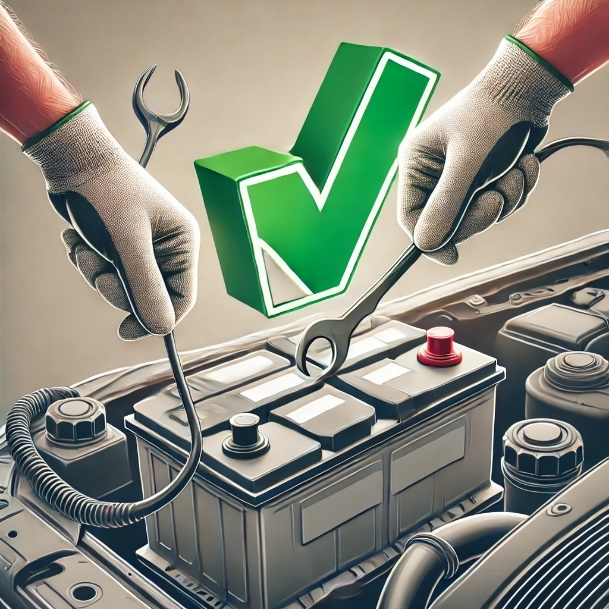
\includegraphics[width=\linewidth]{digifiz_manual/image001.jpg}
        \caption{Наклейка с требованием отключить аккумулятор во время установки.}
    \end{subfigure}\hfill
    \begin{subfigure}{0.46\textwidth}
        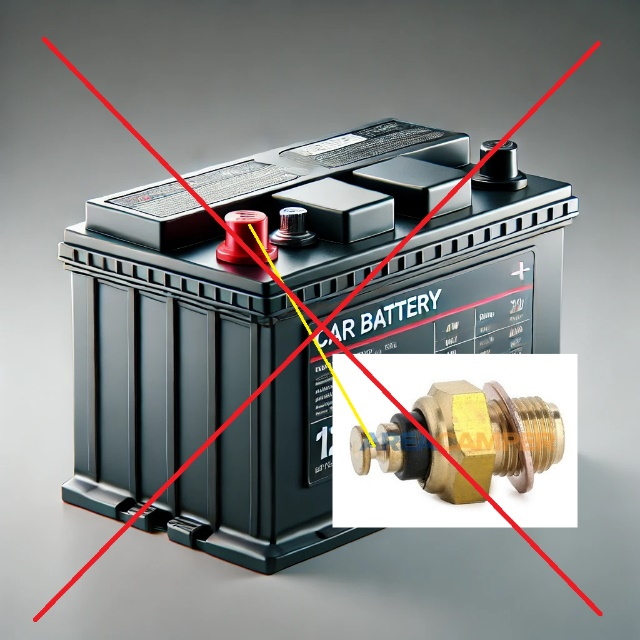
\includegraphics[width=\linewidth]{digifiz_manual/image002.jpg}
        \caption{Предупреждение, прилагаемое к жгуту датчиков, о недопустимости внешнего питания.}
    \end{subfigure}
    \caption{Таблички безопасности, поставляемые с комплектом проводки.}
\end{figure}
